%++++++++++++++++++++++++++++++++++++++++
% Don't modify this section unless you know what you're doing!
\documentclass[letterpaper,12pt]{article}
\usepackage{tabularx} % extra features for tabular environment
\usepackage{amsmath}  % improve math presentation
\usepackage{graphicx} % takes care of graphic including machinery
\usepackage[margin=1in,letterpaper]{geometry} % decreases margins
\usepackage{cite} % takes care of citations
\usepackage[final]{hyperref} % adds hyper links inside the generated pdf file
\hypersetup{
	colorlinks=true,       % false: boxed links; true: colored links
	linkcolor=blue,        % color of internal links
	citecolor=blue,        % color of links to bibliography
	filecolor=magenta,     % color of file links
	urlcolor=blue         
}
%++++++++++++++++++++++++++++++++++++++++

\usepackage{listings}
\usepackage{booktabs}
\usepackage{tabularx}
\usepackage{graphicx}
\usepackage{algorithm}
\usepackage{algorithmic}
\usepackage{float}
\usepackage{graphicx}
\usepackage{wrapfig}
\usepackage[font={small}]{caption}
\usepackage[none]{hyphenat}

\graphicspath{ {./images/}}

\begin{document}

\title{Tabletop MRI Lab Manual}
\author{EE369B: Medical Imaging Systems II}
\date{Winter 2022-23}
%\date{\printdayoff\today}

%%%%%%%%%%%%%%%%%%%%%%%%%%%%%%%%%%%%%%%%%%%%%%%%%%%%%%%%
%%%%%%%%%%%%%%%%%%%%% Front Matter %%%%%%%%%%%%%%%%%%%%%
%%%%%%%%%%%%%%%%%%%%%%%%%%%%%%%%%%%%%%%%%%%%%%%%%%%%%%%%
\maketitle

\tableofcontents

\newpage
\section{Introduction}
The purpose of this lab is to provide hands-on experience with a real MRI scanner to reinforce concepts covered in class. The system you will use is called OCRA: Open-source Console for Real-time Acquisition (Figure \ref{fig:ocra}).

OCRA came together from people all over the world: the MR Physics group at Harvard/MIT created an open-source tabletop scanner; visiting students at MGH translated the technology into a commercial product at the Research Campus STIMULATE of the Otto-von-Guericke University Magdeburg (Germany). Stanford now has three of these systems and we have worked on setting these up as educational tools for the suite of MRI courses offered by the departments of Electrical Engineering and Radiology.

This lab manual will begin by walking you through each component of the OCRA system followed by a brief overview of the basic functionality. Subsequent modules will guide you through exercises in using the scanner to probe a sample.

Take time to familiarize yourself with the components of this scanner. Throughout this lab you are encouraged to explore: if any experimental ideas come up beyond the lab directions, feel free to try these out and add the findings to your report (totally optional). This lab manual is a living document and your input WILL inspire future iterations.

\begin{figure}[h]
    \centering
    %\vspace{-8mm}
    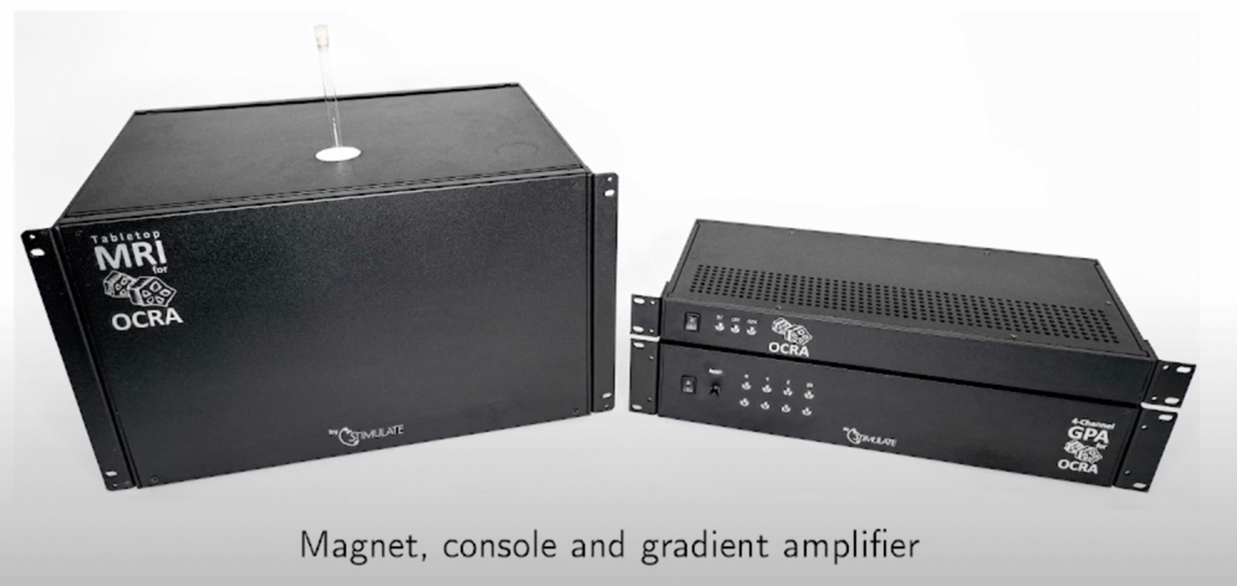
\includegraphics[width=0.9\textwidth]{ocra-system}
    \caption{\label{fig:ocra} OCRA tabletop MRI system including magnet box (left), console (top right) and gradient amplifier (bottom right).}
    \vspace{-5mm}
\end{figure}
\newpage
\section{System Overview}

\begin{wrapfigure}{r}{0.5\textwidth}%this figure will be at the right
    \centering
    \vspace{-2mm}
    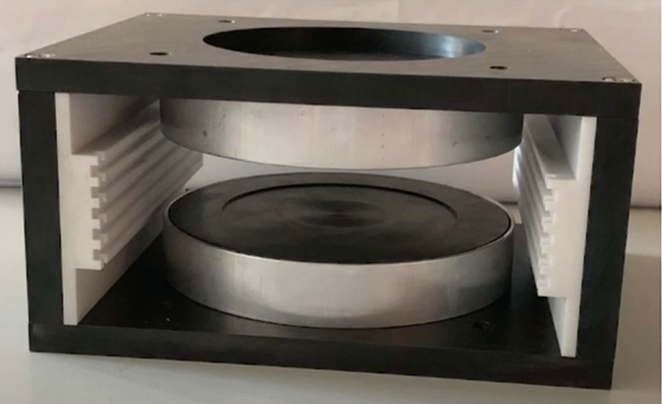
\includegraphics[width=0.48\textwidth]{magnet-interior}
    \caption{\label{fig:magnet} Interior view of the magnet box. Two magnetic disks are held apart with an iron yoke.}
    \vspace{-10mm}
\end{wrapfigure}

There are several components associated with the OCRA tabletop MRI scanner. The primary components are described as follows: 
\vspace{5mm} 

\noindent\textbf{Magnet:} The B0 field is created by a small 0.26T permanent magnet (Figure \ref{fig:magnet}). Two rare-earth magnetic disks are held apart with an iron yoke. The yoke also provides a flux-return path for the magnetic field, containing the magnetic field to the gap between the two poles (and inside the iron). 
\vspace{5mm} 

\noindent\textbf{Phantoms:} A small hole in the top of the magnet serves to accommodate imaging samples. The term \emph{phantom} is used to describe artificial imaging targets.  Next to the scanner you will find several glass tubes to serve as phantoms for this lab.
\vspace{5mm} 

\noindent\textbf{RF coil:}
A radio-frequency (RF) coil encircles the sample bore, serving to transmit the excitation pulse and detect the MR signal through the Faraday detection principle. \textbf{The coil is sensitive to a 20 mm FOV along the bore, centered 15 mm above the bottom of the bore hole}. The coil is a simple solenoid built into an electrical resonator with parallel capacitance so it can be tuned to a specific Larmor frequency. The coil is enclosed by an RF shield consisting of 4 printed circuit boards (PCBs) soldered edge-to-edge (Figure \ref{fig:rf-coil}). The shield acts as a Faraday cage to protect surrounding electronics from RF radiation.

 \begin{figure}[h]
    \centering
    %\vspace{-8mm}
    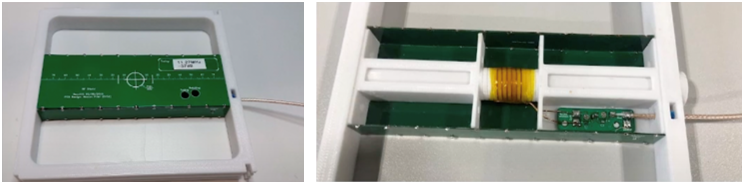
\includegraphics[width=0.9\textwidth]{rf-coil}
    \captionsetup{width=.9\textwidth}
    \caption{\label{fig:rf-coil} (Left) 4 PCBs encase the RF coil to protect surrounding electronics. (Right) RF coil solenoid inside the RF shield.}
    \vspace{-5mm}
\end{figure}

\vspace{5mm}

\noindent\textbf{RF Box:} Inside the magnet box, an RF box (Figure \ref{fig:rf-box-and-grad-filter}, left panel) contains several RF-related components including an RF amplifier, transmit-receive switch, and first \& second stage pre-amplifiers for the received MR signal.  The transmit-receive switch is used to connect the RF coil to the RF amplifier (transmit mode) or low noise pre-amplifier (receive mode).

 \begin{figure}[h]
    \centering
    %\vspace{-8mm}
    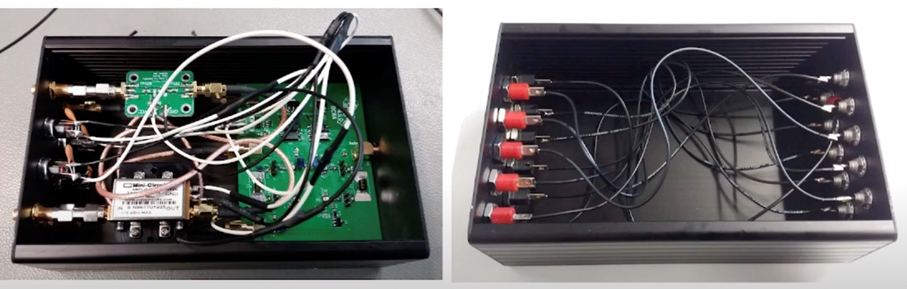
\includegraphics[width=0.9\textwidth]{rf-box-and-grad-filter}
    \caption{\label{fig:rf-box-and-grad-filter} RF box (left) and gradient filter box (right). Both reside in the magnet box.}
    \vspace{-2mm}
\end{figure}

\vspace{5mm}

\noindent\textbf{Gradient System:} The gradient system includes PCB coils, an amplifier, and filter circuitry. The gradient coils (Figure \ref{fig:grad-coils}) generate a spatially varying magnetic field proportional to the current supplied by the amplifier.

\begin{wrapfigure}{r}{0.5\textwidth}%this figure will be at the right
    \centering
    %\vspace{-2mm}
    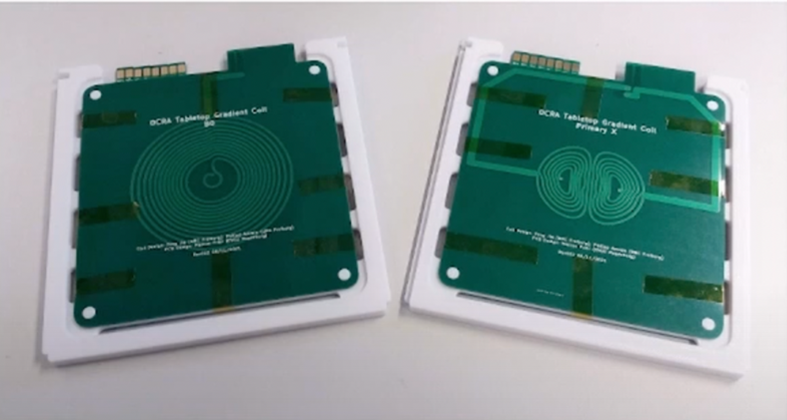
\includegraphics[width=0.48\textwidth]{grad-coils}
    \caption{\label{fig:grad-coils} PCB gradient coils.}
    %\vspace{-5mm}
\end{wrapfigure}

\vspace{5mm}

The gradient amplifier (Figure \ref{fig:grad-amp}) can be viewed as a voltage-to-current transducer: it takes a voltage waveform from the console and creates a current proportional to that voltage in the gradient coil. It is like a common audio power amplifier except that it must also be able to output DC currents.

The gradient amplifier support four channels (X, Y, Z, Z2). The additional channel Z2 is used not for imaging but rather for maintaining homogeneity of the magnetic field.

The amplifier box includes current protection to protect the coils and temperature protection to protect the end stage of each channel. There is also a large power supply and printed circuit boards for the amplifiers.

Filter circuitry (Figure \ref{fig:rf-box-and-grad-filter}, right panel) resides in its own box inside the magnet box, with connections to the gradient channels and feed-through capacitors to shield noise from the gradient amplifier.

\begin{figure}[h]
    \centering
    %\vspace{-8mm}
    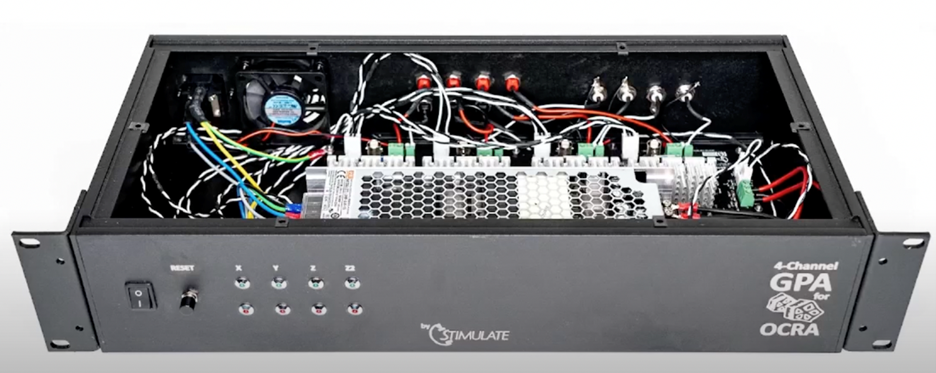
\includegraphics[width=0.9\textwidth]{grad-amp}
    \captionsetup{width=.9\textwidth}
    \caption{\label{fig:grad-amp} Gradient amplifier with X, Y, Z and Z2 channels.}
    \vspace{-2mm}
\end{figure}

\vspace{5mm}

\noindent\textbf{Console:} The console box (Figure \ref{fig:console}) contains two primary components: a Red Pitaya micro-controller and an Ocra1 board (Figure \ref{fig:console-boards}). The Red Pitaya interfaces with a basic MRI console and coordinates signal acquisition by generating RF pulses and control signals for the transmit-receive switch. The MR signal picked up by the RF coil is sampled at an RF input channel through the integrated analog-to-digital converter (RX) on the Red Pitaya. The Red Pitaya is connected to the Ocra1 board which has four 18-bit digital-to-analog converters for gradient waveform generation and an RF attenuator to scale the Red Pitaya output for the RF amplifier input. The console also contains the power supply and a circuit responsible for distributing power among the different parts.

Figure \ref{fig:comms-overview} illustrates the communication pathways between the Red Pitaya, Ocra1, and Raspberry Pi (to be introduced below).

\begin{figure}[h]
    \centering
    %\vspace{-8mm}
    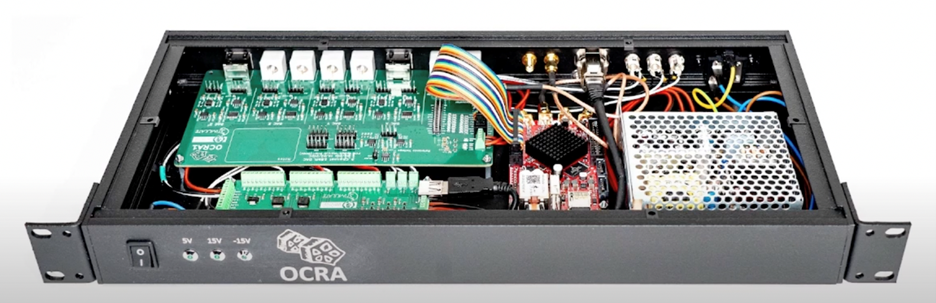
\includegraphics[width=0.9\textwidth]{console-interior}
    \caption{\label{fig:console} Interior view of the console box housing the Red Pitaya micro-controller and the Ocra1 board.}
    \vspace{-5mm}
\end{figure}

\begin{figure}[h]
    \centering
    %\vspace{-8mm}
    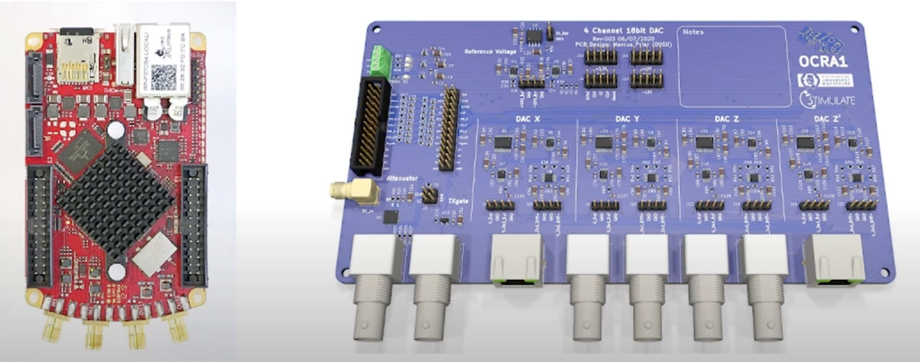
\includegraphics[width=0.7\textwidth]{red-pitaya-and-ocra1}
    \caption{\label{fig:console-boards} Red Pitaya microcontroller (left) and Ocra1 board (right) outside of the RF box.}
    \vspace{-5mm}
\end{figure}

\vspace{5mm} 

\noindent\textbf{Graphical User Interface (GUI):} A Raspberry Pi single-board computer (not pictured - you can find it sitting behind the OCRA stack) allows the user to interface with the tabletop scanner. It hosts a Python program \emph{Relax 2.0} that provides a GUI to interface with the Red Pitaya micro-controller. Basically this program translates Python sequence instructions into RF transmit pulses and gradient waveforms for the lower level hardware to implement.

\begin{figure}[h]
    \centering
    %\vspace{-8mm}
    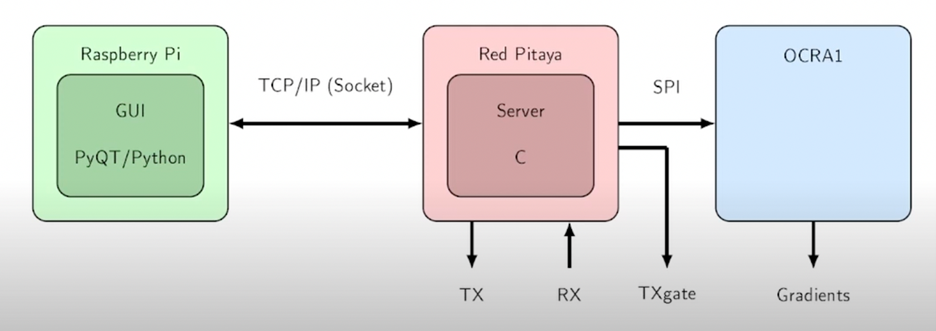
\includegraphics[width=0.9\textwidth]{comms-overview}
    \captionsetup{width=.9\textwidth}
    \caption{\label{fig:comms-overview} Overview of connections between the Raspberry Pi, Red Pitaya, and Ocra1. The Raspberry Pi provides the GUI for the user to change sequence parameters and interact with the system. The Raspberry Pi communicates to the Red Pitaya via a TCP/IP Socket. The OCRA1 extends the Red Pitaya to a basic MRI console via serial peripheral interface (SPI) bus given by the RP GPIO pins. The Red Pitaya coordinates data acquisition by generating RF pulses (TX) and control signals for the transmit-receive switch (TXgate).}
    \vspace{-5mm}
\end{figure}
\newpage
\section{Basic Functionality}

\subsection{VNC Access} \label{sec:vnc}

We use the graphical desktop-sharing system \href{https://en.wikipedia.org/wiki/Virtual_Network_Computing}{VNC} to manage access to the tabletop systems. VNC should be used for both in-person and remote work.

\begin{enumerate}
    \item   Install a free VNC application such as \href{https://tigervnc.org/}{tigervnc}.
    \item   Ensure you are connected to the Stanford network (use VPN if off-campus).
    \item   \label{step:login} Use VNC to connect to one of the tabletop systems using the login information below. Figure \ref{fig:vnc} shows an example.
    \begin{itemize}
        \item   User: Ocra1, VNC: mrtabletop:1, Pitaya IP: 192.168.1.84, password: Initpw123
        \item   User: Ocra2, VNC: mrtabletop:2, Pitaya IP: 192.168.1.83, password: Initpw123
        \item   User: Ocra3, VNC: mrtabletop:3, Pitaya IP: 192.168.1.82, password: Initpw123
    \end{itemize}
\end{enumerate}

\begin{wrapfigure}{r}{0.4\textwidth}
    \centering
    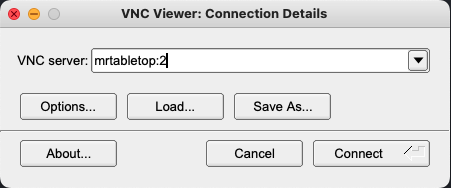
\includegraphics[width=0.36\textwidth]{vnc-example}
    \captionsetup{width=.36\textwidth}
    \caption{\label{fig:vnc}Example of a VNC connection interface.}
\end{wrapfigure}

Troubleshooting tips:
\begin{itemize}
    \item   Make sure you are the only person logged into the machine that you are trying to use. The machines won’t respond well if multiple users are using them and running sequences simultaneously.
    \item   If at any point the Pitaya stops responding or the sequences don’t run properly, you can restart the Pitaya remotely via the following steps:
    \begin{enumerate}
        \item   From the mrtabletop machine, ssh in to the appropriate Pitaya with the command \texttt{ssh root@192.168.1.xx}. (replace xx with IP suffix from step \ref{step:login}). There shouldn’t be a password prompt.
        \item   Once you are logged in, run the command \texttt{reboot}. The Pitaya will automatically restart and your ssh session will be terminated.
        \item   After the Pitaya reboots try running a simple test sequence. An easy sequence to run as a debugging step is a spin-echo.
    \end{enumerate}
\end{itemize}

% \subsection{System Start-up}

% \emph{Under normal circumstances the tabletop system will be powered on already and you can skip ahead to section \ref{sec:relax-program}.}

% Before beginning the startup procedure, ensure all boxes in the OCRA stack are OFF and the Raspberry Pi is unplugged.

% \begin{enumerate}
%     \item Switch the console box \textbf{on}.
%     \item Switch the gradient amplifier \textbf{on}. Press and hold the \textbf{Reset} button until the indicator lights turn green.
%     \item Plug in the Raspberry Pi. Login with password \texttt{raspberry}.
%     %\item Navigate to \texttt{/home/pi/Relax2} and double-click on \texttt{Relax2\_main.py} to open. Click the green arrow in the code editor to run the program.
%     %\item A dialog box will appear prompting you to select an IP address. Use the default IP address and click \textbf{Connect}.
%     %\item Observe the Relax 2.0 main menu (Figure \ref{fig:gui-menu}).
% \end{enumerate}

\begin{wrapfigure}{r}{0.4\textwidth}%this figure will be at the right
    \centering
    %\vspace{-15mm}
    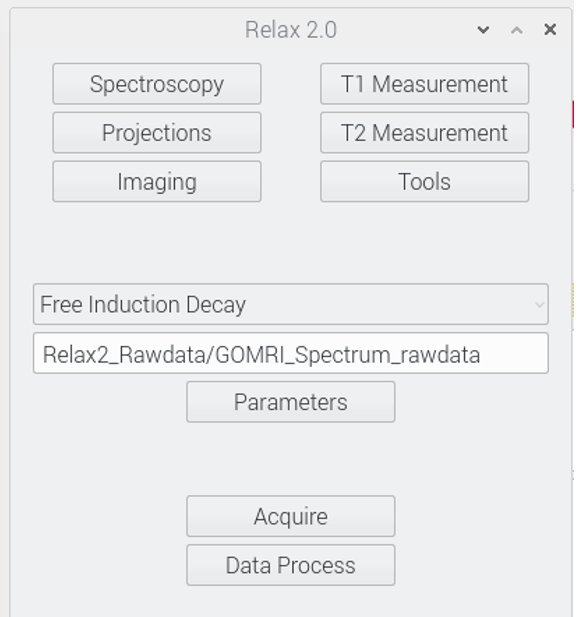
\includegraphics[width=0.36\textwidth]{gui-menu}
    \captionsetup{width=.36\textwidth}
    \caption{\label{fig:gui-menu}Relax 2.0 main menu.}
    %\vspace{-10mm}
\end{wrapfigure}

\subsection{Relax 2.0 Program} \label{sec:relax-program}

To run the Relax 2.0 program:

\begin{enumerate}
    \item   Open a terminal window.
    \item   Navigate to the program directory:
    
    \texttt{cd /home/ocra\#/Documents/221120\_Relax2}
    
    (\emph{replace \# appropriately})

    \item   Run the program:
    
    \texttt{python Relax2\_main.py}.

    \item   Enter the appropriate IP address (refer to section \ref{sec:vnc}).
    
\end{enumerate}

The Relax 2.0 main menu (Figure \ref{fig:gui-menu}) is the starting point for all experiments in this lab. The top 6 buttons toggle between broad categories of scans such as spectroscopy and projection imaging. The drop-down menu lists specific pulse sequences within the selected scan category. A typical workflow involves picking a category and a sequence, then modifying the sequence parameters over a series of acquisitions. These latter operations are explained below.

\textbf{Parameters} opens a window listing all mutable sequence parameters (e.g. echo time TE, repetition time TR) \emph{for all possible sequences}. Note that many of these parameters many not actually be used for a given sequence. This is an idiosyncrasy of the program that can be confusing. The lab manual should always tell you exactly which parameters to modify, but if there is any ambiguity don't hesitate to ask.

\textbf{Acquire} runs the selected sequence with the current parameter set. Unlike most scanners, expect this to run \emph{silently}.

\textbf{Data Process} operates on the raw data captured by the most recent \textbf{Acquire} event, calling any reconstruction and post processing routines associated with the selected sequence.

\subsection{Data Export}
\noindent{}In this lab you will capture experimental outputs in the form of screenshots and/or text files.

With a VNC connection you can capture screenshots of the remote desktop view with your own computer. This will be the primary mechanism for documenting your progress through the lab (e.g. saving plots and images), so make sure you have this working smoothly before you begin.

% \emph{Without a VNC connection}, if you access the Raspberry Pi directly then screenshots can be captured by opening a terminal window and using the \texttt{scrot} command. For example, \texttt{scrot filename.png} will save a screenshot to \texttt{filename.png} in the current working directory. Append a path to \texttt{filename.png} if you would like to specify some other directory.

Raw data and image data (if saved) are written to text files in the folders \texttt{Relax2\_Rawdata} and \texttt{Relax2\_Imagedata} folders respectively, both located in the same directory as \texttt{Relax2\_main.py}. You can change the folder or filename to prevent overwrite by editing the path in the field below the drop-down menu.

Finally, you can use a USB drive to transfer any files on the Raspberry Pi to another computer. To this end there will be one USB drive available for use \emph{in lab}. Please take care to erase the drive and leave it next to the phantom tray at the end of each session.


%%%%%%%%%%%%%%%%%%%%%%%%%%%%%%%%%%%%%%%%%%%%%%%%%%%%%%%%
%%%%%%%%%%%%%%%%%%%%%%% Modules %%%%%%%%%%%%%%%%%%%%%%%%
%%%%%%%%%%%%%%%%%%%%%%%%%%%%%%%%%%%%%%%%%%%%%%%%%%%%%%%%
\newpage
\section{Lab Modules}
\newpage
\subsection{Calibration}

An ideal MR scanner should exhibit perfect homogeneity in the static field $B_0$, RF transmit field $B_1^+$, and perfect linearity in the gradient fields. Moreover, RF pulses should be perfectly matched to the Larmor frequency of the sample. In practice, no scanner can achieve all these characteristics perfectly. Calibration serves to minimize these discrepancies to promote signal quality.

This module will guide you through calibrating the tabletop scanner in three stages: finding the Larmor frequency of a sample, tuning the RF pulse amplitude to achieve a $90^{\circ}$ tip angle, and shimming (flattening) the $B_0$ field. \textbf{The Larmor frequency calibration is particularly sensitive to environmental changes and should be repeated periodically during each lab session.} Shimming and RF tuning need only be completed once as an exercise for this module.

\textbf{Use a water-only phantom for this module.}

\subsubsection{Finding the Center Frequency} \label{sec:center}

\noindent{}\textbf{Note: this frequency calibration is extremely sensitive to temperature. It is recommended to re-calibrate the center frequency every 10-20 minutes or before any important scan.}
\vspace{3mm}

The \emph{center frequency} describes the carrier frequency for RF excitation pulses as well as the demodulation frequency for signal reception. In both cases we want the center frequency calibrated to the Larmor frequency of the target nuclei at the magnet \emph{isocenter} (point where all gradients are zero). If the center frequency is poorly calibrated, then excitation is said to be off-resonance and the basic tip angle behavior $\theta = \gamma B_1 \tau$ does not hold.
% Spins \emph{may} still become excited (to a lesser degree) but the excited profile will not be as straight-forward.

For $^1 H$ imaging with this 0.26T scanner, the nominal Larmor frequency is: 

$$ f = \frac{\gamma}{2\pi} B_0 = 42.58\,\text{MHz/T} \times 0.26\,\text{T} = 11.1\,\text{MHz} $$

The current center frequency of the tabletop scanner is available in the \textbf{Parameters} menu under \emph{General}, labelled ``RF Frequency [MHz]''. Make a note of this current value to track how it changes over the course of calibration. This is a good practice whenever you are re-calibrating the center frequency.

Relax 2.0 provides two methods for calibrating the center frequency: a coarse search when the error is large, and fine-tuning when the error is small. First let's try the fine-tuning method, which aims to center the frequency spectrum of the received signal.

 \begin{figure}[h]
    \centering
    \vspace{-5mm}
    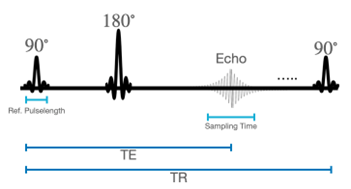
\includegraphics[width=0.7\textwidth]{spin-echo}
    \captionsetup{width=.9\textwidth}
    \caption{\label{fig:calib-spin-echo} Sequence diagram for a non-selective spin echo sequence used to calibrate the center frequency. No gradients are active. The echo envelope is determined by T2* decay.}
    %\vspace{-5mm}
\end{figure}

\begin{enumerate}
    \item In the main menu, click \textbf{Spectroscopy} and select the \textbf{Spin Echo} sequence from the drop-down menu. This sequence is depicted in Figure \ref{fig:calib-spin-echo}.
    \item \label{step:params} Open the \textbf{Parameters} menu. Set the following parameters: under \emph{General} set TE to 10 ms, TR to 2000 ms, Sampling Time to 6 ms; under \emph{Config \& Misc} set 90 Ref. RF Pulse Length to 100 $\mu$s, RF Attenuation to -10 dB.
    \item \label{step:acquire} Return to the main menu. Click \textbf{Acquire}. Wait for the spin echo sequence to run.
    \item \label{step:process} Click \textbf{Data Process}. Observe the two resulting figures plotting the received signal in time and frequency domains. Note these plots show the received signal \emph{after demodulation} by the current center frequency. Try adjusting the frequency range in the Plotvalues window to zoom in on the peak. This can help visualize any bias in the center frequency.
    \item \label{step:recenter} Calibrate the center frequency by navigating to the \textbf{Parameters} menu and clicking \textbf{Recenter} under the center frequency field. % This will update the center frequency according to the bias of the resonant peak in the frequency spectrum. TODO check code to see if this is actually how it works
    \item Repeat steps \ref{step:acquire} to \ref{step:recenter}. A well-calibrated center frequency should result in a sharp peak at 0 in the (demodulated) frequency spectrum. Also, there should be minimal exchange between the real \& imaginary parts in the time domain plot. Thus you can use these two plots to visually assess the quality of your calibration. If the results are poor, try repeating this step once more. If the results are still poor then do the coarse search method below for a better initial value.
\end{enumerate}

If the fine-tuning method was unsuccessful, try the coarse search method. The approach here is to iterate over different center frequencies and record the peak signal, which should be highest at the Larmor frequency.

\begin{enumerate}
    \item Use the same timing parameters as for the fine-tuning method (step \ref{step:params} above).
    \item Navigate to the main menu. Click \textbf{Tools} and locate the \emph{AutoCenter} tool.
    \item Find the note on the magnet box with an approximate center frequency for this particular magnet (e.g. 11.25 MHz).
    \item Set the \emph{AutoCenter} start \& end frequencies to span a 0.1 MHz range centered on the value you found noted on the magnet box. Set the iteration step size to 5000 Hz.
    \item Click \textbf{Go}. The AutoCenter tool will take a few minutes to run. 
    \item When the tool finishes, navigate to the \textbf{Parameters} menu and update the center frequency by clicking the \textbf{Set to Tool Ref} button under the RF Frequency field.
    \item Try the fine-tuning method again.
\end{enumerate}

\noindent{}\color{red}When you are satisfied with the calibration result, capture a screenshot of the two figure windows alongside the Plotvalues window reporting center frequency, FWHM, SNR, and B0 inhomogeneity. These are useful metrics for understanding signal quality. It is a good practice to pay attention to how these values change over the course of calibration.
\color{black}

\subsubsection{RF Attenuation}

The RF Attenuation calibration adjusts the RF Pulse Amplitude to achieve a $90^{\circ}$ tip angle.

\begin{enumerate}
  \item Navigate to the main menu. Click \textbf{Spectroscopy} and select \textbf{Spin Echo} from the drop-down menu. Use the same parameters as in \ref{sec:center}.
  \item Navigate to the main menu. Click \textbf{Tools} and locate the \emph{TrAdj} (Transmit Adjust) tool. Set the attenuation range to [-20, -1] dB with 20 steps. 
  \item Click \textbf{Go}. This will take a minute to run.
  \item When the tool is finished, you will see a plot of signal vs RF attenuation. A $90^{\circ}$ tip angle is achieved where the signal is maximal. This value is reported in the Tools window in the Ref Attenuation field.
  \item Set RF attenuation to this value in the \textbf{Parameter} menu. This can be done automatically by clicking \textbf{Set to Tool Ref} under the RF Attenuation field. 
  \item Run the Spectroscopy Spin Echo sequence again (\textbf{Acquire}) and visualize the result (\textbf{Data Process}). Your signal should be improved. Re-center the center frequency as it may have shifted.  
\end{enumerate}

\noindent{}\color{red}Screenshot the RF attenuation plot. Report the value you find for RF Attenuation to achieve $90^{\circ}$ tip angle.
\vspace{5mm}

\noindent{}\color{red}Capture a screenshot of your improved spin-echo spectrum. What do you notice is different than before? You can also reference statistics from the Plotvalues window for comparison.
\color{black}

\subsubsection{Shimming} 

\noindent{}Shimming is used to improve homogeneity of the main field $B_0$. We do this by adding small, constant currents (DC) to each of the gradient coils. The Z2 channel is exclusively used for shimming whereas the other three gradients X/Y/Z also serve to enable spatial localization, as we will see in upcoming modules.

\vspace{5mm}

\noindent{} Maximizing the homogeneity of the magnetic field corresponds to narrowing the frequency spectrum of a pure sample. Hence we can evaluate the quality of shimming by measuring the height and width of a pure sample's resonant peak in the frequency spectrum. The spectral area should be constant (proportional to number of protons magnetized), so improving the field homogeneity should result in a higher peak with smaller FWHM (full width at half maximum).

\vspace{5mm}

\noindent{} Shimming can be quite time-consuming, so we have already shimmed these systems for you. Instead of having you repeat this entire process, we will have you re-do the shim calibration for just one of the gradients to understand the process and observe the effect on signal quality.

\begin{enumerate}
  \item Find the current shim settings in \textbf{Parameters} under \emph{Config \& Misc}.
  \noindent{}\color{red} Record the current shim settings for Shim X, Shim Y, Shim Z, and Shim Z2. 
  \color{black}
  \item Shift the Shim X value by 50 mA.
  \item \label{step:spin-echo} Run a spectroscopy spin echo (same as you did previously to find the center frequency). You should find that the change to Shim X worsens (increases) the B0 inhomogeneity.
  
  \noindent{}\color{red} Capture a screenshot of the resulting plots.
  \color{black}
  \item Click \textbf{Tools} and locate the \emph{Shim} tool section. This tool serves to test different shim values for a selected gradient. 
  \item Select the X gradient in the tool menu. Set the range of values to span 100 mA centered on the original value of Shim X you recorded above. Set the number of steps to 20.
  \item Click \textbf{Go}. This will take a minute.
  \item After the tool runs you will see a plot of signal versus shim value.
  
    \noindent{}\color{red}
  Capture a screenshot of this plot.
  \color{black}
  \item Repeat the above process once more with a refined range of 10 values spanning 10 mA centered on the optimal value you found from the first run.
  \item The shim value for which peak signal is achieved will be reported in the tool window. Update the Shim X value in the \textbf{Parameters} menu accordingly.
  
  \color{black}
     \noindent{}\color{red}
  Report the optimal Shim X value you found.
  \color{black}
  \item Repeat step \ref{step:spin-echo}.
\end{enumerate}

\noindent{}\color{red} Comment on the difference in signal quality (e.g. B0 inhomogeneity) between the three shim settings: initial state (before calibration), shifted by 50 mA, and after calibration.
\color{black}

Throughout this lab you will want to keep B0 inhomogeneity below 50 ppm to ensure reasonably accurate measurements. You can always check this value by acquiring a spectroscopy spin echo and inspecting the Plotvalues window.
\vspace{5mm}

\noindent{} This concludes the calibration module. You have a working scanner! Now is a good time to clean up the desktop as you have likely accrued many windows. You can clear all program windows at once by simply terminating the Relax 2.0 Python program.





\newpage
\subsection{Spectroscopy}

In this module we study a few of the basic MR signals that can be measured with one or two RF pulses and no gradients. \textbf{Use a water-only phantom for this module}.

\subsubsection{Free Induction Decay} \label{sec:fid}

The most basic MR signal is the Free Induction Decay (FID). An FID results from the action of a single RF pulse, presenting as a damped oscillation of the excited transverse magnetization (Figure \ref{fig:FID}). 

\vspace{5mm}

\noindent{}\color{red}
What is the oscillation frequency for the FID? What mechanism(s) are responsible for damping this oscillation?
\color{black}
% soln: oscillates at the Larmor frequency, damped by T2* decay (which itself is a combination of T2 decay and dephasing due to off-resonance)

\begin{figure}[h]
    \centering
    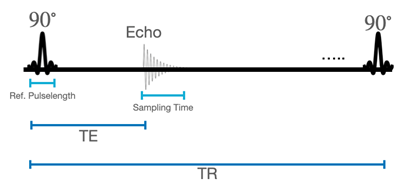
\includegraphics[width=0.7\textwidth]{free-induction-decay}
    \captionsetup{width=.9\textwidth}
    \caption{\label{fig:FID} Pulse sequence inducing free induction decay (FID). A single RF pulse produces a damped oscillation in the transverse magnetization signal.}
\end{figure}

\noindent{Follow these steps to measure an FID signal:} 
\begin{enumerate}
    \item   In the main menu, click \textbf{Spectroscopy} and select the \textbf{Free Induction Decay} sequence.
    \item	Open \textbf{Parameters}. Under \emph{General} set TE to 5 ms, Sampling Time to 6 ms.
    \item	Click \textbf{Acquire}, then \textbf{Data Process}. 

Observe the resulting figures. These plots depict the FID signal in time and frequency domain after demodulation by the center frequency. Hence if the center frequency is well-calibrated you should not see much oscillation, only decay.

    \item Try acquiring a few more FIDs at larger echo times TE.

\end{enumerate}

\subsubsection{Spin Echo}

Another basic MR signal is the Spin Echo. You may have already measured a spin echo in a previous module (e.g. for calibration). Nevertheless we review it here for the purpose of comparison with FID. A spin echo results from the action of two RF pulses, separated by a time TE/2 (Figure \ref{fig:spec-spin-echo}). The spin echo occurs at echo time TE.

\vspace{5mm}

\noindent{}\color{red}
What is the oscillation frequency of a spin echo signal? What mechanism(s) are responsible for shaping the envelope of this oscillation?
\color{black}

\begin{figure}[h]
    \centering
    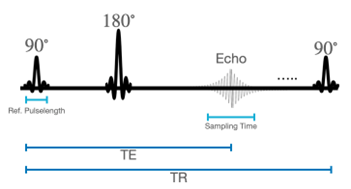
\includegraphics[width=0.7\textwidth]{spin-echo}
    \captionsetup{width=.9\textwidth}
    \caption{\label{fig:spec-spin-echo} Pulse sequence inducing a spin echo at echo time TE. Two RF pulses work to excite then refocus the transverse magnetization signal.}
\end{figure}
\vspace{5mm}

\noindent{Follow these steps to measure a Spin Echo signal:}
\begin{enumerate}
\item	Navigate to the main menu. Click \textbf{Spectroscopy} and select the \textbf{Spin Echo} sequence.
\item	Open \textbf{Parameters}. Under \emph{General} set TE to 10 ms, Sampling Time to 6 ms.
\item	Click \textbf{Acquire}, then \textbf{Data Process}.
\item Try acquiring a few more spin echoes at larger echo times TE.
\end{enumerate}

Observe the resulting figures. As with the FID signal, these plots depict the received signal in time and frequency domains after demodulation by the center frequency, hence the oscillation depicted in Figure \ref{fig:spec-spin-echo} should be largely removed.

\vspace{5mm}

\noindent{}\color{red}
How does the spin echo signal change as you increase TE? Compare with what you observed when you increased TE for the FID signal. Explain the difference.
\color{black}

\vspace{5mm}

\noindent{}\color{red}
Capture screenshots of the resulting plots for both FID and Spin Echo at a few different values of TE.
\color{black}

\newpage
\subsection{Projection Imaging}

In this module we begin to explore imaging with the MR scanner by introducing spatial encoding along one dimension. We do this by adding a single gradient to the spin echo spectroscopy sequence used in previous modules. Playing this gradient during readout enables spatial discrimination along the gradient dimension. The resulting data can then be reconstructed into a 1D image by means of Fourier transformation, with the other two orthogonal dimensions being projected. Alternatively, additional projections may be acquired to resolve a higher-dimensional image, e.g. like the back-projection algorithm does for x-ray computed tomography (CT).

Figure \ref{fig:grad-axes} shows the OCRA naming convention for the gradient axes. The $x$ axis points to the right, the $y$ axis points up, and the $z$ axis points forward. This agrees with the conventional MR nomenclature \emph{in the lab frame}. However keep in mind that relative to the bore axis the $y$ and $z$ axes are actually swapped compared with convention. It's all a matter of perspective, isn't it?

\begin{wrapfigure}{r}{6cm}
    \centering
    \vspace{-10mm}
    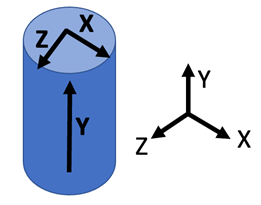
\includegraphics[width=6cm]{grad-axes}
    \caption{\label{fig:grad-axes} OCRA naming convention for gradient axes with sample bore in blue.}
    \vspace{-10mm}
\end{wrapfigure}

\subsubsection{Water Phantom}
Use a water-only phantom for this portion of the experiment. You will measure projections along the $x$, $y$, and $z$ axes.

\begin{enumerate}
    \item   Navigate to the main menu. Click \textbf{Projections} and select \textbf{Spin Echo (On Axis)}.
    \item   Open \textbf{Parameters}. Under \emph{General}, set TE to 10 ms, TR to 2000ms, Sampling Time to 6 ms. Under \emph{Imaging}, set Image Resolution to 64 and FOV to 30 mm. Under \emph{Projections}, select X, Y, and Z to iterate through each gradient axis one at a time.
    \item   Click \textbf{Acquire}, then \textbf{Data Process}.
\end{enumerate}

Observe the resulting plots of frequency spectra in $x$, $y$, and $z$. Adjust the frequency range to better visualize the profile. The 2D image plot is XZ plane and is reconstructed from only these three basic projections, hence the result is very crude.

\noindent{}\color{red}
Save a screenshot of the spectral plots and comment on their appearance.
\color{black}

\subsubsection{Mystery (?) Phantom}
Now you will repeat the above experiment to probe a mystery phantom. The mystery phantom is labelled with a question mark. It contains one or more water-filled holes oriented along $y$. Your task is to use projection imaging to deduce the number of water-filled holes in this phantom. Hint: try rotating the phantom to capture different projection angles.

\noindent{}\color{red}
How many holes are in the mystery phantom? Explain your reasoning and include screenshots to support your conclusion. 
\color{black}
\newpage
\subsection{2D Imaging}

In this module we recruit two gradient channels to enable imaging in two spatial dimensions. To do this we will use the basic 2DFT sequence you have learned about in class.

Implementation of a 2DFT sequence requires that we specify the amplitude and duration of gradient waveforms. These parameters follow from the imaging prescription, i.e. field-of-view (FOV) and resolution. Let us recall a few concepts from class to elucidate this design calculation.

\begin{enumerate}
    \item   The time integral of an encoding gradient tells us where we are in sampling k-space along the axis corresponding to that gradient. In equation form, we have
    \begin{equation}
        k(t)=\frac{\gamma}{2\pi} \int_{0}^{t} G(\tau) d\tau
    \end{equation}
    \item   The extent of coverage in one domain (object or k-space) corresponds to the reciprocal of resolution in the transform domain. In equation form, we have
    \begin{equation}
        \Delta k=\frac{1}{FOV}; \; k_{max}=\frac{1}{2\Delta x}
    \end{equation}
\end{enumerate}

Now with a concrete example we can combine these equations to design the gradient parameters. Say we want a 256 mm FOV and 2 mm resolution ($\delta$). Assume the hardware provides a perfect rectangle waveform and the sampling period $\Delta t$ is 30 $\mu$s. Combining the above equations yields the following readout amplitude $G_{xr}$ and duration $\tau_x$ for readout along $x$.

\begin{equation*}
    G_{xr}=\frac{1}{\frac{\gamma}{2\pi} \text{FOV}_x \Delta t} \approx 3 \; \text{mT/m}
\end{equation*}

\begin{equation*}
    \tau_x=\frac{1}{\frac{\gamma}{2\pi}G_{xr} \delta_x} \approx 4 \; \text{ms}
\end{equation*}

A similar calculation can be done for the phase encoding gradient but we will not review that here. For the exact equations you can refer to pages 86 and 90 of the textbook\footnote{Nishimura, Dwight G. \emph{Principles of Magnetic Resonance Imaging}, Lulu.com, 2010.}.

The Relax 2.0 program computes gradient parameters in a similar manner as shown above, with the added step of calculating the current necessary to achieve the gradient strength. In the following sections you will not have to repeat the above calculations, but it is important to understand how these values are computed behind the scenes.

\subsubsection{Spin Echo} \label{sec:spin-echo}

In previous modules you used a spin echo sequence for spectroscopy (no gradients) and projection imaging (one gradient during readout). Now we will use it for 2D imaging, by adding a second gradient to perform phase encoding prior to each readout. In this way each readout can acquire a different line of k-space.

\vspace{5mm}

\noindent{}\color{red}

Sketch the pulse sequence diagram for a 2DFT spin echo pulse sequence.
\vspace{5mm}

Consider the effect of swapping axes for readout and phase encode gradients. How does the k-space trajectory change? Would the image change? Explain.

\color{black}

\vspace{5mm}

\emph{As a reminder, you should re-center the RF Frequency if you have not done so recently (see Calibration module, use the Spectroscopy Spin Echo, etc).}

\vspace{5mm}

Now let's get to imaging!

\begin{enumerate}
    \item Insert the gray star phantom.
    \item Navigate to the main menu. Click \textbf{Imaging} and select the \textbf{2D Spin Echo} sequence.
    \item Open \textbf{Parameters}. Under \emph{General}, set TE to 10 ms, TR to 1000 ms, Sampling Time to 6 ms. Under \emph{Imaging}, set Image Orientation to ZX, Image Resolution to 64 pixels, FOV to 30 mm.
    \item Click \textbf{Acquire}. This sequence takes a long time to run because it takes many repetitions to fill 2D k-space at just one line per excitation.
    
\noindent{}\color{red}
Propose 3 sequence modifications that could reduce the scan time. Hint: you will not have to implement these changes so you need not limit yourself to the options available in the GUI.
\color{black}  

    \item When the sequence finishes, click \textbf{Process Data}. You will then see a 2x2 grid of magnitude and phase images for both k-space and the object domain.

\noindent{}\color{red}Include a screenshot of the resulting spin echo images. Comment on the image quality and any notable features you observe, such as k-space structure or image artifacts, if any exist.
\noindent{}\color{black}

    \item Change the Image Resolution to 128 pixels and run the sequence again.

\noindent{}\color{red}
Include a screenshot of the resulting images. Compare image quality with the previous lower resolution image and explain any difference besides resolution.
\noindent{}\color{black}

    %\item Change the FOV and Image Resolution to a different combination and run the sequence again.

%\noindent{}\color{red}Q: Comment on the changes you observe with this third parameter set. Did your changes positively or negatively affect image quality? Why?
\color{black}

\end{enumerate}

\subsubsection{Gradient Echo}
Now we will run a 2D gradient echo sequence for comparison. 

\begin{enumerate}
\item	Use the same water shape phantom as you did for the spin echo section above.
\item   Navigate to the main menu. Click \textbf{Imaging} and select the \textbf{2D Gradient Echo} sequence.
\item   Use the same parameters as in \ref{sec:spin-echo} (reverting Image Resolution back to 64 pixels).
\item   Click \textbf{Acquire}. This will take about as long as the 2D spin echo sequence.
\item   When the sequence finishes, click \textbf{Process Data}.
\end{enumerate}

\noindent{}\color{red}Include a screenshot of the resulting gradient echo images. Comment on how these images compare with the spin echo images you acquired before and explain any differences. Hint: recall the spectroscopy module, where you compared FID with spin echo.

Propose a change in sequence parameters that could improve the gradient echo image and explain any trade-offs.
\noindent{}\color{black}
% soln: shorten the echo time and sampling time. Tradeoff between SNR and T2* dephasing. Worthwhile in this case because B0 inhomogeneity is severe, so T2* dephasing is dominant.

\newpage
\subsection{Relaxometry} \label{sec:relax}

The time evolution of magnetization towards equilibrium is characterized by relaxation time constants $T_1$ and $T_2$ for longitudinal and traverse components, respectively. In biological tissues, dipole-dipole interactions serve as the dominant mechanism responsible for relaxation. Field strength and material composition modulate dipole-dipole interactions, hence a wide range of $T_1$ and $T_2$ values can be found for the same nuclear target, e.g. ${}^1 H$.

In this module you will explore several methods for measuring the $T_1$ and $T_2$ of a few basic tissue-mimicking materials. Table \ref{table:relax} lists these materials with empirical measurements of $T_1$ and $T_2$ \textbf{at 1.5 T} from recent literature\footnote{Antoniou, Anastasia, et al. ``MR relaxation times of agar‐based tissue‐mimicking phantoms.'' Journal of Applied Clinical Medical Physics 23.5 (2022): e13533.}.

\begin{table}[!h]
\begin{center}
\begin{tabular}{ |c|c|c| } 
\hline
\textbf{Material} & \textbf{$T_1$ (ms)} & \textbf{$T_2$ (ms)} \\ \hline
Oil & 193 & 55 \\ \hline
Agar & 1670 & 46 \\ \hline
\end{tabular}
\end{center}
\caption{\label{table:relax} Mean $T_1$ and $T_2$ of basic tissue-mimicking materials for proton (${}^1 H$) imaging at 1.5T.}
\end{table}

Note the field strength at which the measurements in Table \ref{table:relax} were collected. In most biological tissues, $T_1$ increases approximately as $B_0^{1/3}$ and $T_2$ is approximately constant over the range of field strength relevant to clinical MRI.

\vspace{5mm}

\color{red} Use the $B_0^{1/3}$ power law and Table \ref{table:relax} to estimate $T_1$ of oil and 2\% agar at the field strength of the tabletop system (0.26T).
\color{black}
% soln:
% T1 * (0.26/1.5)^(1/3)
% oil 108ms; agar 931ms; water 1185ms

\vspace{5mm}

\begin{wrapfigure}{r}{0.5\textwidth}
    \vspace{-5mm}
    \centering
    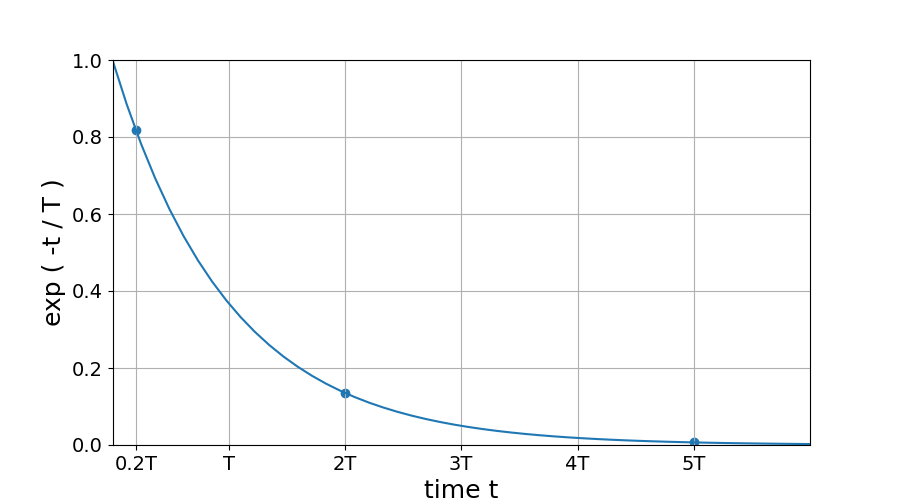
\includegraphics[width=0.5\textwidth]{exp-decay}
    \captionsetup{width=0.4\textwidth}
    \caption{\label{fig:decay} Exponential decay with a generic time constant $T$. This plot can be a helpful reference for designing relaxometry experiments.}
\end{wrapfigure}

In order to measure $T_1$ or $T_2$ you will tune the timing parameters of a spin echo sequence to elicit sensitivity to just one of these time constants at a time. For the sake of both accuracy and efficiency, it will be important to \textbf{design your sampling range to cover the most significant portion of the decay/recovery curve} for the time constant you are measuring. To this end you may find Figure \ref{fig:decay} to be a helpful reference for choosing parameters in proportion to the (expected) time constant value. For example, we can see that the majority of decay/recovery happens during the time window between 20\% and 200\% of the time constant T. By time 5T, decay is practically complete.

\newpage
\subsubsection{Measuring $T_2$} \label{sec:T2}

\emph{Note: B0 homogeneity is very important for $T_2$ measurement accuracy. Check that B0 inhomogeneity is below 50 ppm before continuing. You can check this value by acquiring a spectroscopy spin echo and inspecting the Plotvalues window.}

\vspace{5mm}
Consider the following saturation-recovery spin echo sequence.
\newline \newline
$90^{\circ}$ --- TE/2 --- $180^{\circ}$ --- TE/2 --- DAQ
\newline \newline
We will use this sequence to measure $T_2$ by iterating over a range of echo times (TE) and fitting a mono-exponential to the resulting signal decay curve $s(\text{TE})$. The Relax 2.0 program will actually do this for you by fitting a line to the log of the decay curve.
\vspace{5mm}

\color{red}
Derive an expression for $T_2$ in terms of the slope of the linearized decay, $\log{s}$. Assume complete recovery over each iteration ($\text{TR} \gg T_1$).
\color{black}
\vspace{5mm}
% soln: $T_2 = -1 / slope$

We will now collect data to plot the decay curve and measure $T_2$ for a sample.

\begin{enumerate}
    \item   Install the oil phantom. \emph{Remember to re-calibrate the center frequency as needed}.
    \item   In the main menu, click \textbf{T2 measurement} and select the \textbf{Spin Echo} sequence.
    \item  Open \textbf{Parameters}. Under \emph{General}, set Sampling Time to 6 ms and pick a suitable TR for $T_1$ insensitivity. Under \emph{T2 Measurement}, choose a suitable range of 10 TE values for fitting a $T_2$ decay.
    \item   Click \textbf{Acquire} and wait for the program to run its course.
    \item   Click \textbf{Data Process} and observe the resulting plot.
    \item   Tune your timing parameters as needed to achieve a good fit ($|r| \geq 0.97$). Hint: Figure \ref{fig:decay} can help you pick suitable values for TE and TR.

    \color{red} Report your chosen timing parameters and explain your reasoning.
    \color{black}
    % soln: avoid T_1 contrast with TR >> T_1; TE range around T_2$

    \color{red} 
    Include a screenshot of the resulting plot with $T_2$ and $r$ clearly visible. 
    \color{black}

    \color{red} 
    Use the formula you derived for the slope to validate the $T_2$ value computed by Relax 2.0. Comment on the agreement with Table \ref{table:relax}.
    \color{black} 
    
    % works well with TE range around 10-200% of T2
    \item   Repeat these steps for each material in Table \ref{table:relax}.
\end{enumerate}

\color{red}
You may have noticed that TE values much larger than $T_2$ tend to produce outliers in the linear fit. Explain this effect.
\color{black}
% soln: as transverse signal decays to 0, thermal noise becomes dominant and we lose the mono-exponential shape

\newpage
\subsubsection{Measuring $T_1$} \label{sec:T1}

Consider the following inversion-recovery spin echo sequence. We will use this sequence to measure $T_1$ by iterating over a range of inversion times (TI). \newline
\newline
$180^{\circ}$ --- TI --- $90^{\circ}$ --- TE/2 --- $180^{\circ}$ --- TE/2 --- DAQ
\newline

\color{red}
Sketch the $M_z$ magnetization for one iteration of this sequence, assuming $\text{TR} \gg T_1$. Use your sketch to derive an expression for the $M_z$ null point in terms of $T_1$. Hint: the $M_z$ null point is the time at which $M_z$ crosses through zero after the initial $180^{\circ}$ pulse. 
\color{black}
% soln: TI_null = T_1 log(2) (eqn 7.51 in Nishimura textbook)

We will now collect data to locate the $M_z$ null point for a sample and measure $T_1$:
\begin{enumerate}
    \item   Install the oil phantom. \emph{Remember to re-calibrate the center frequency as needed}.
    \item   In the main menu, click \textbf{T1 measurement} and select \textbf{Inversion Recovery (SE)}.
    \item   Open \textbf{Parameters}. Under \emph{General}, set Sampling Time to 6 ms, pick a suitable TE for $T_2$ insensitivity, and pick a suitably long TR for full recovery. Under \emph{T1 Measurement}, choose a suitable range of 10 TI values to locate the $M_z$ null point.
    \newline
    \color{red} Report your chosen timing parameters and explain your reasoning.
    \color{black}
    % soln: TR >> T_1; TE << T_2; TI range should include expected null-point at T_1 log(2)$
    \item   Click \textbf{Acquire} and wait for the program to run its course.
    \item   Click \textbf{Data Process} and observe the resulting plots. Ignore the fit lines and reported $T_1$ value for now - these will likely be way off.
    \newline
    \color{red}
    Record the approximate TI value achieving minimum signal amplitude among the 10 points. Take this TI value as the $M_z$ null point to estimate $T_1$ using the formula you derived above.
    \color{black}
    % soln: T_1 = TI_null / log(2)

    \item Finally, we will measure $T_1$ again but this time by fitting a mono-exponential to the recovery curve. The \textbf{Data Process} routine actually does this for you by fitting a line to the log of the recovery curve $s(\text{TI})$. To be precise, the Relax 2.0 software actually fits a line to $\log{(\text{max}(s)-|s|)}$. This is a rather precarious implementation choice, but it should work well enough for our purpose so long as the following conditions are met:
    \begin{itemize}
        \item TI range begins \emph{after} the $M_z$ null point
        \item $\text{max}(s)$ is close to the equilibrium magnetization, i.e. $\text{max}(\text{TI}) \gg T_1$
    \end{itemize}
    
    With these conditions in mind, tune your timing parameters to achieve a good fit ($|r| \geq 0.97$) with 10 values for TI. One more hint: choose TR such that $\text{TR} - \text{max}(\text{TI}) \gg T_1$ to ensure adequate signal recovery in all cases.
        
\color{red}
Report your chosen timing parameters and explain your reasoning.
\color{black}
% works well with TI range 100-500% of T1

\color{red}
Attach screenshots of the two resulting plots with $T_1$ and r-value clearly visible.
\color{black}
% soln: In addition to the guidance provided in the hints (TI_max >> T1, TR - TI_max >> T1), want TE << T2 and TI spanning the significant portion of the recovery curve.

    \item   Repeat these steps for each material in Table \ref{table:relax}.

\end{enumerate}

\color{red}
Now you have tried three different methods for estimating $T_1$ in a variety of materials. Comment on the degree of agreement and relative accuracy across these methods.
\color{black}






\newpage
\subsection{Multi-compartment Imaging} \label{sec:multi}

In this final module you will integrate everything you have learned in this lab to probe a multi-compartment phantom using spectroscopy, projections, and 2D imaging.

\textbf{Use the agar + oil phantom throughout this module.}

%\textbf{Use the water + oil phantom until directed otherwise}. Please take care to keep this phantom upright so as to preserve the separation of water and oil.

\vspace{5mm}
\noindent \emph{Re-calibrate the center frequency before any lengthy imaging sequence for best image quality.}

% \begin{wrapfigure}{r}{0.5\textwidth}
%     \vspace{-5mm}
%     \centering
%     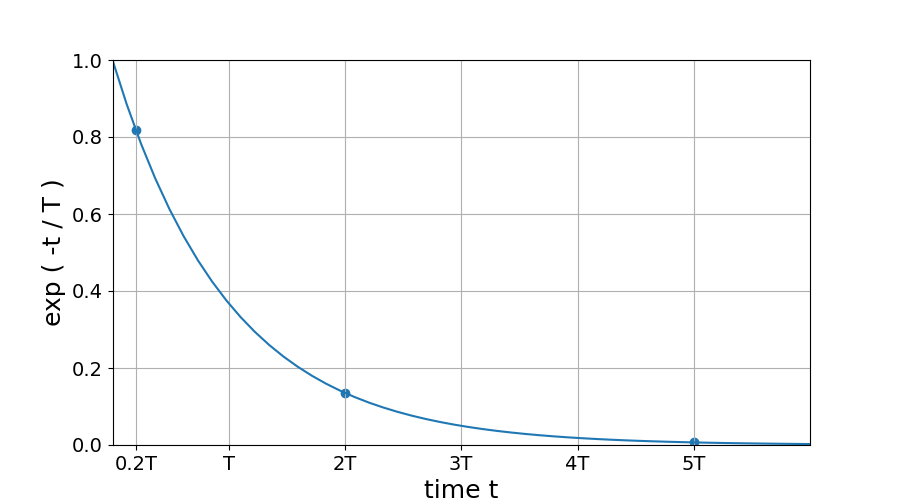
\includegraphics[width=0.5\textwidth]{exp-decay}
%     \captionsetup{width=0.4\textwidth}
%     \caption{\label{fig:decay} Exponential decay with a generic time constant $T$. This plot can serve as a reference for designing efficient relaxometry experiments.}
% \end{wrapfigure}



\subsubsection{Spectroscopy}

We begin by inspecting the spin echo spectrum for this multi-compartment phantom.

\begin{enumerate}
\item	In the main menu, click \textbf{Spectroscopy} and select the \textbf{Spin Echo} sequence.
\item	Open \textbf{Parameters}. Under \emph{General} set TE to 10 ms, Sampling Time to 6 ms.
\item	Click \textbf{Acquire}, then \textbf{Data Process}.
\end{enumerate}

\color{red}
\noindent You learned in class that the resonant frequency of fatty tissue (oil here) differs from watery tissue (agar here) due to an electron shielding effect called chemical shift. Why do we only see one peak in the spectrum? How \emph{could} this experiment be modified to resolve the two peaks (without changing the phantom itself)? Hint: your answer may well go beyond the current capabilities of the tabletop system by changing/improving hardware or software.
\color{black}
% soln: increase sampling time to improve spectral resolution, but also need better B0 homogeneity for this to actually help. Or, use a stronger main field to increase the spectral separation. Or introduce a gradient to spatially resolve the two, then rely on contrast (e.g. T1, T2) to separate.

\subsubsection{Projection with $T_2$ Contrast} \label{sec:proj-T2}

%Now let's play with the signal contrast of two materials having significantly different $T_2$: water and oil.
Now let's begin to play with $T_2$ contrast:

\begin{enumerate}
    \item   In the main menu, click \textbf{Projections} and select the \textbf{Spin Echo (On Axis)} sequence.
    \item   Open \textbf{Parameters}. Under \emph{General}, set TE to 10 ms, Sampling Time to 6 ms. Under \emph{Imaging}, set Image Resolution to 64 and FOV to 30 mm. Under \emph{Projections}, select only Y (the bore axis).
    \item   Click \textbf{Acquire}, then \textbf{Data Process}.
    \item   Observe the resulting projection plot. Adjust the frequency range to better visualize the signal profile. You should find that the two materials are nearly indistinguishable with these timing parameters.
    \item   Now try repeating the scan for several larger values of TE to increase the contrast. Do not change any other parameters. Observe how the relative signal levels change between the two materials.
\end{enumerate}

\color{red} \noindent
Include screenshots of the projection plot for three values of TE showing a range of contrast from low to high.
\color{black}
\vspace{5mm}

\color{red}
\noindent
Explain why these values of TE lead to different contrasts. Derive an expression for the optimal TE maximizing $T_2$ contrast between any two materials. Use the $T_2$ values you measured in the relaxometry module to compute the optimal TE for this case. How does this optimal TE compare with what you found empirically?
\color{black}
% soln: TE = log(T2_oil / T2_agar) / (1/T2_agar - 1/T2_oil)

\subsubsection{2D Imaging with $T_2$ Contrast} \label{sec:2d-T2}

Now that you have achieved $T_2$ contrast, let's see how it looks in a 2D image.

\begin{enumerate}
    \item   In the main menu, click \textbf{Imaging} and select the \textbf{2D Spin Echo} sequence.
    \item   Open \textbf{Parameters}. Under \emph{General}, set TR to 5000 ms, Sampling Time to 6 ms. Set TE for maximal T2 contrast between the two materials (use what you found in section \ref{sec:proj-T2}). Under \emph{Imaging}, set Image Orientation to XY, Image Resolution to 32 pixels, FOV to 30 mm.
    \item   Click \textbf{Acquire}. After it runs, click \textbf{Data Process}.
    \item   Observe the resulting images. \emph{If you are using ocra1 you will find the image y axis is flipped relative to the lab frame (bright agar appears on top).}
    \item   Repeat the above steps for a different TE value exhibiting minimal contrast.
    
    \color{red} Screenshot the resulting images for both TE values.
    \color{black}
 
    \item Repeat one of the above scans with Sampling Time 1 ms and 12 ms.

\color{red} \noindent
    Compare the set of images with different sampling times. Explain any differences. Hint: in order to cover the same k-space extent the readout gradient amplitude must be inversely proportional to the sampling time.
\color{black}
    
\end{enumerate}


\subsubsection{2D Imaging with $T_1$ Contrast} \label{sec:2d-T1}

% Try repeating section \ref{sec:proj-T2} with an agar + oil phantom (no write-up necessary). You will find it is much harder to distinguish agar \& oil because the $T_2$ value are more similar. Hence we will explore $T_1$ weighting as an alternative means of contrast for this phantom.

Now we will explore $T_1$ weighting as an alternative means of contrast for this phantom.

\begin{enumerate}
    \item   In the main menu, click \textbf{Imaging} and select the \textbf{2D Spin Echo} sequence.
    \item   Open \textbf{Parameters}. Under \emph{General}, set TE to 10 ms, Sampling Time to 6 ms. Under \emph{Imaging}, set Image Orientation to XY, Image Resolution to 32 pixels, FOV to 30 mm.
    \item   Design TR values to achieve (i) no contrast and (ii) high contrast between the two materials. Use the $T_1$ values you measured in the relaxometry module to inform your design. \emph{Note: the Relax 2.0 software limits TR to a minimum of 500 ms.}
 \end{enumerate}

 \color{red} \noindent
 Include screenshots of the resulting images with no/high $T_1$ contrast.
 \color{black}

\subsubsection{2D Imaging with $T_1$ Nulling} \label{sec:2d-T1}

Fat signal can be a nuisance for clinical MRI, so many techniques have been developed to remove this signal. One such approach is called TI-nulling. This approach uses an inversion recovery (IR) sequence with the inversion time (TI) parameter tuned to suppress a particular $T_1$ species. We will use this approach to suppress the ``fat'' signal in this phantom.

\color{red}
Calculate the TI needed to null the oil signal using the $T_1$ you measured in the relaxometry module. Hint: you should have already derived the necessary equation for this calculation in the relaxometry module. Your sketch of the sequence may also be helpful to reference.
\color{black}
% soln: TI=T1*log(2)
% around 70 ms

\begin{enumerate}
    \item   Navigate to the main menu. Click \textbf{Imaging} and select the \textbf{2D Inversion Recovery (SE)} sequence.
    \item   Open \textbf{Parameters}. Under \emph{General}, set TE to 10 ms, set TI to the fat-nulling value you found, Sampling Time to 6 ms, TR to 5000 ms. Under \emph{Imaging}, set Image Orientation to XY, Image Resolution to 32 pixels, FOV to 30 mm.
    \item   Click \textbf{Acquire}. After it runs, click \textbf{Data Process}.
 \end{enumerate}

\noindent{}\color{red}
Include a screenshot of the fat-suppressed images.
\color{black}



%\newpage
\subsection{K-space Manipulation}
If we have time in class, you may begin this section. We will be working with a brain dataset and looking at what happens when we manipulate the k-space and undersample it. Acquiring one line of k-space at a time we have seen in the previous section can be very slow and tedious and would be a very long scan if we collected many slices and a high-resolution in vivo. In this section we will simulate different ways of undersampling the data and its effect on the image output.

\subsubsection{Matlab Code}
A small Matlab script has been provided. It is a live notebook, so you can load individual cells and the resultant images that may appear are below. Please have the .mat data file and the script in the same folder.  


\subsubsection{Undersampling K-space}
Instead of acquiring undersampled data, we will modify this dataset and “simulate” undersampling conditions. In other words, we can create “mask” matrices that consist of 1s and 0s and multiply it with our k-space data to simulate undersampling. This will delete the lines with the 0s and keep the ones with 1s. 

\vspace{5mm} 

\noindent{} Run the Matlab Code for the undersampling section with the following masking instructions:

\vspace{5mm} 
 
\noindent{}\color{red}Q: Zero every other row in k-space and display the resultant k-space and the image. Comment on the image you reconstruct.

\color{black}
\vspace{5mm} 

\noindent{}\color{red}Q: Zero every other column in k-space and display the resultant k-space and the image. Comment on the image you reconstruct.
\color{black}

\vspace{5mm} 

\noindent{}\color{red}Q: Zero 2/3 of the k-space columns (keep one column, zero 2 columns) and display the resultant k-space and the image. Comment on the image you reconstruct.
\color{black}

\subsubsection{Lowpass/ High Pass Filters}
K-space is the 2D spatial frequency domain. Different frequenies encodes different types of information. We are going to investigate the role of low and high frequencies in the reconstruction of an image. We can isolate the two components by designing filters that keep only the frequencies we are interested in. Low-pass filters remove all the high frequencies leaving only low frequencies, and High-pass filters perform in the opposite manner. Therefore, we will apply a low-pass and high-pass filter to the image. Follow the directions in the questions below and include figures in your lab writeup. 
  
\vspace{5mm} 

\noindent{}\color{red}Q: Zero the center 50\% of the k-space. Take the inverse Fourier transform and display your image. Comment on how this image compares to the original. 
\color{black}

\vspace{5mm} 

\noindent{}\color{red}Q: Zero the outer 50\% of the k-space. Take the inverse Fourier transform and display your image. Comment on how this image compares to the original. 
\color{black}

\vspace{5mm} 


\end{document}